% \documentclass[12pt]{extarticle}

% \usepackage[margin=0.75in]{geometry}
% \usepackage{inputenc}
% \usepackage[tbtags]{amsmath}
% \usepackage{amsfonts}
% \usepackage{graphicx}
% \usepackage{amsmath}

% \begin{document}

% \section*{\centering Demystifying $d_0$ \\
% \section*{Demystifying the Impact Parameter ($d_0$) \\
% \small J. Rosenzweig \\ 
% \small 2020-01-30
% }



% MAYBE DON'T INCLUDE ANY \section or \subsection content!
% Only use \chapter !

% TODO: Clean all this up!
\chapter{Ad hoc impact parameter studies}
\label{app:adhoc_studies}

% \chapter{The sign of impact parameter}
% \label{app:qd0_derivation}

Consider a reconstructed muon track projected onto the $xy$ plane, transverse to the beam pipe.
If the muon was a prompt muon, then it truly originated from the primary vertex (PV).
However, due to inefficiencies in reconstructing the muon track, 
the best-fit track may not intersect the PV. 

Looking at Figure~\ref{fig:traj} (Left), the (very exaggerated) muon track is represented by the black circle.
This track could either be a $\mu^+$ (blue arrowheads) travelling around clockwise, since the magnetic field points along the $+\hat{z}$ direction,
or it could represent the track of a $\mu^-$ (orange arrowheads) travelling anticlockwise.

It is convenient to define a few variables:
\begin{itemize}
    \item $\vec{s} =$ the field point vector which begins at the PV (the origin) and ends at the point-of-closest-approach (PCA) along the muon track.
    \item $\phi_s =$ the azimuthal angle of ${\vec{s}}$ as measured from the $x$-axis.
    \item $\phi_{\mu^{\pm}} =$ the azimuthal angle of the $\vec{p}_{T,\mu^{\pm}}$, tangent to the track at the PCA, measured from the $x$-axis.
\end{itemize}

% field point vector $(\vec{s})$ begins at the PV (the origin) and ends at the point-of-closest-approach (PCA) along the muon track.

%%%%%%%%%%%%%%%%%%%%
\begin{figure}[bpht]
% \begin{figure}[b]
    \centering
    \includegraphics[width=\textwidth,keepaspectratio]{../../higgsmassmeasurement/AN-19-248/Figures/adhoc_d0/PV_outside_vs_inside.png}
        \caption
            [Hello faculty! Yes, I see this ugly Appendix formatting---I will fix ASAP.]
            {(Left) The case in which the true primary vertex (PV) is \emph{outside} the circular trajectory of a muon.
            (Right) The opposite case in which the PV is \emph{inside} the circular trajectory. 
            } 
        \label{fig:traj}
\end{figure}
%%%%%%%%%%%%%%%%%%%%

From Fig.~\ref{fig:traj} (Left) we see that:
\begin{equation}
    \label{azimuth}
\phi_{\mu^{\pm}} = \phi_{s} \pm \pi/2.
\end{equation}
Using one possible definition of $d_{0}$ and Equation~\ref{azimuth} shows that 
the $d_0$ for $\mu^{\pm}$ which came from a PV outside the circle trajectory is:
\begin{align*}
    d_{0,\mu^{\pm}}^{\text{PV,outside}} &= -x \sin{( \phi_{\mu^{\pm}} )}  + y \cos{( \phi_{\mu^{\pm}} )} \\
    &= - x \sin{( \phi_s \pm \pi/2 )} + y \cos{( \phi_s \pm \pi/2 )}  \\
    &= -x \big[ \sin{(\phi_s)} \cos{(\pi/2)}  \pm \sin{(\pi/2)} \cos{(\phi_s)} \big]  
       + y \big[\cos{(\phi_s)} \cos{(\pi/2)} \mp \sin{(\phi_s)} \sin{(\pi/2)} \big] \\
    &= - x [\pm \cos{(\phi_s)}] + y [\mp \sin{(\phi_s)}] \\
    &= \mp [x \cos{(\phi_s)}  + y \sin{(\phi_s)}] \\
    &= \mp \big[ x \hat{x} + y \hat{y}  \big] \boldsymbol{\cdot} \big[ \cos(\phi_{s}) \hat{x} + \sin(\phi_{s}) \hat{y}  \big] \\
    &= \mp \vec{s} \boldsymbol{\cdot} \hat{s} \\
    &= \mp \lvert \vec{s} \rvert   \lvert \hat{s} \rvert    \cos{(0)}
\end{align*}
\begin{equation}
    \label{eqn:d0_out}
    \implies  d_{0,\mu^{\pm}}^{\text{PV,outside}} = \mp \lvert \vec{s} \rvert. 
\end{equation}

The case for the PV being {\it inside} the circle trajectory (Fig.~\ref{fig:traj}, Right) simply leads to a sign change in Eqn.~\ref{azimuth}:
\begin{equation}
    \label{azimuth_flipped}
\phi_{\mu^{\pm}} = \phi_{s} \mp \pi/2.
\end{equation}
Starting again from the definition of $d_0$, but this time using Eqn.~\ref{azimuth_flipped}, ultimately gives:
\begin{equation}
    \label{eqn:d0_in}
\implies  d_{0,\mu^{\pm}}^{\text{PV,inside}} = \pm \lvert \vec{s} \rvert.
\end{equation}

Indeed we see that the magnitude of $d_0$ {\it is the transverse impact parameter} $(\lvert \vec{s} \rvert)$, as expected!
The sign of $d_0$, however, is not possible to interpret at this point: 
for a $d_0 > 0$ could either mean a $\mu^-$ coming from a PV outside the circlular trajectory \emph{or}
could mean a $\mu^+$ coming from a PV found inside the circle.

Since the sign of $d_0$ is not useful by itself, consider multiplying $d_0$ by the charge of its corresponding muon. 
We then see that Eqn.~\ref{eqn:d0_out} becomes:
\begin{align*}
    {\rm charge}(\mu^{\pm}) \cdot d_{0,\mu^{\pm}}^{\text{PV,outside}} &= \pm1 \cdot \mp \lvert \vec{s} \rvert \\
    &= - \lvert \vec{s} \rvert < 0,
\end{align*}
which is always negative. Similarly, Eqn.~\ref{eqn:d0_in} gives the opposite result:
\begin{equation*}
    {\rm charge}(\mu^{\pm}) \cdot d_{0,\mu^{\pm}}^{\text{PV,inside}} = + \lvert \vec{s} \rvert > 0,
\end{equation*}
which of course is always positive. 

Therefore, if we know the sign of the muon (say, negative) 
and the sign of its $d_0$ (say, positive), 
then we can simply take the product (negative in this case) 
and infer that the PV must have been \emph{outside} the muon trajectory!

To summarize: it is the \emph{product} of the charge and $d_0$ that contains useful information about the muon track. 
\[
    {\rm PV} = 
\begin{cases}
    \text{inside of circle},& \text{if charge}(\mu^{\pm}) \cdot d_{0,\mu^{\pm}} > 0 \\
    \text{outside of circle},& \text{if charge}(\mu^{\pm}) \cdot d_{0,\mu^{\pm}} < 0.
\end{cases}
\]
% \end{document}

%---------------%
% \newpage
\chapter{Correlation between transverse momentum bias and impact parameter}
% \label{app:dpT_graphs}

\begin{figure}[!htbp]
    % \vspace*{0.3cm}
    \centering
    { \includegraphics[width=0.47\textwidth]{../../higgsmassmeasurement/AN-19-248/Figures/adhoc_d0/dpToverpTvsqd0_graphs_2017/graph_dpTvsqd0_0p0eta0p2.png}}
    { \includegraphics[width=0.47\textwidth]{../../higgsmassmeasurement/AN-19-248/Figures/adhoc_d0/dpToverpTvsqd0_graphs_2017/graph_dpTvsqd0_0p2eta0p4.png}}
    { \includegraphics[width=0.47\textwidth]{../../higgsmassmeasurement/AN-19-248/Figures/adhoc_d0/dpToverpTvsqd0_graphs_2017/graph_dpTvsqd0_0p4eta0p6.png}}
    { \includegraphics[width=0.47\textwidth]{../../higgsmassmeasurement/AN-19-248/Figures/adhoc_d0/dpToverpTvsqd0_graphs_2017/graph_dpTvsqd0_0p6eta0p8.png}}
    { \includegraphics[width=0.47\textwidth]{../../higgsmassmeasurement/AN-19-248/Figures/adhoc_d0/dpToverpTvsqd0_graphs_2017/graph_dpTvsqd0_0p8eta1p0.png}}
    { \includegraphics[width=0.47\textwidth]{../../higgsmassmeasurement/AN-19-248/Figures/adhoc_d0/dpToverpTvsqd0_graphs_2017/graph_dpTvsqd0_1p0eta1p3.png}}
    { \includegraphics[width=0.47\textwidth]{../../higgsmassmeasurement/AN-19-248/Figures/adhoc_d0/dpToverpTvsqd0_graphs_2017/graph_dpTvsqd0_1p3eta1p5.png}}
    \caption{ 
        Graphs of \pTmismeas vs. avg$(\qdzero)$ for each \abseta bin using 2017 MC.
        The \abseta bin edges shown above are: $[0.0, 0.2, 0.4, 0.6, 0.8, 1.0, 1.25, 1.5]$.
        Each line uses data from a single \pT bin. 
        The \pT correction parameters for each (\abseta, \pT) bin are found in the legend.
    }
\end{figure}
\newpage
\begin{figure}[!htbp]
    % \vspace*{0.3cm}
    \centering
    { \includegraphics[width=0.47\textwidth]{../../higgsmassmeasurement/AN-19-248/Figures/adhoc_d0/dpToverpTvsqd0_graphs_2017/graph_dpTvsqd0_1p5eta1p8.png}}
    { \includegraphics[width=0.47\textwidth]{../../higgsmassmeasurement/AN-19-248/Figures/adhoc_d0/dpToverpTvsqd0_graphs_2017/graph_dpTvsqd0_1p8eta2p0.png}}
    { \includegraphics[width=0.47\textwidth]{../../higgsmassmeasurement/AN-19-248/Figures/adhoc_d0/dpToverpTvsqd0_graphs_2017/graph_dpTvsqd0_2p0eta2p1.png}}
    { \includegraphics[width=0.47\textwidth]{../../higgsmassmeasurement/AN-19-248/Figures/adhoc_d0/dpToverpTvsqd0_graphs_2017/graph_dpTvsqd0_2p1eta2p2.png}}
    { \includegraphics[width=0.47\textwidth]{../../higgsmassmeasurement/AN-19-248/Figures/adhoc_d0/dpToverpTvsqd0_graphs_2017/graph_dpTvsqd0_2p2eta2p3.png}}
    { \includegraphics[width=0.47\textwidth]{../../higgsmassmeasurement/AN-19-248/Figures/adhoc_d0/dpToverpTvsqd0_graphs_2017/graph_dpTvsqd0_2p3eta2p4.png}}
    \caption{ 
        Graphs of \pTmismeas vs. avg$(\qdzero)$ for each \abseta bin using 2017 MC.
        The \abseta bin edges shown above are: $[1.5, 1.75, 2.0, 2.1, 2.2, 2.3, 2.4]$.
        Each line uses data from a single \pT bin. 
        The \pT correction parameters for each (\abseta, \pT) bin are found in the legend.
    }
\end{figure}

\newpage
\begin{figure}[!htbp]
    % \vspace*{0.3cm}
    \centering
    { \includegraphics[width=0.47\textwidth]{../../higgsmassmeasurement/AN-19-248/Figures/adhoc_d0/dpToverpTvsqd0_graphs_2018/graph_dpTvsqd0_0p0eta0p2.png}}
    { \includegraphics[width=0.47\textwidth]{../../higgsmassmeasurement/AN-19-248/Figures/adhoc_d0/dpToverpTvsqd0_graphs_2018/graph_dpTvsqd0_0p2eta0p4.png}}
    { \includegraphics[width=0.47\textwidth]{../../higgsmassmeasurement/AN-19-248/Figures/adhoc_d0/dpToverpTvsqd0_graphs_2018/graph_dpTvsqd0_0p4eta0p6.png}}
    { \includegraphics[width=0.47\textwidth]{../../higgsmassmeasurement/AN-19-248/Figures/adhoc_d0/dpToverpTvsqd0_graphs_2018/graph_dpTvsqd0_0p6eta0p8.png}}
    { \includegraphics[width=0.47\textwidth]{../../higgsmassmeasurement/AN-19-248/Figures/adhoc_d0/dpToverpTvsqd0_graphs_2018/graph_dpTvsqd0_0p8eta1p0.png}}
    { \includegraphics[width=0.47\textwidth]{../../higgsmassmeasurement/AN-19-248/Figures/adhoc_d0/dpToverpTvsqd0_graphs_2018/graph_dpTvsqd0_1p0eta1p3.png}}
    { \includegraphics[width=0.47\textwidth]{../../higgsmassmeasurement/AN-19-248/Figures/adhoc_d0/dpToverpTvsqd0_graphs_2018/graph_dpTvsqd0_1p3eta1p5.png}}
    \caption{ 
        Graphs of \pTmismeas vs. avg$(\qdzero)$ for each \abseta bin using 2018 MC.
        The \abseta bin edges shown above are: $[0.0, 0.2, 0.4, 0.6, 0.8, 1.0, 1.25, 1.5]$.
        Each line uses data from a single \pT bin. 
        The \pT correction parameters for each (\abseta, \pT) bin are found in the legend.
    }
\end{figure}
\newpage
\begin{figure}[!htbp]
    % \vspace*{0.3cm}
    \centering
    { \includegraphics[width=0.47\textwidth]{../../higgsmassmeasurement/AN-19-248/Figures/adhoc_d0/dpToverpTvsqd0_graphs_2018/graph_dpTvsqd0_1p5eta1p8.png}}
    { \includegraphics[width=0.47\textwidth]{../../higgsmassmeasurement/AN-19-248/Figures/adhoc_d0/dpToverpTvsqd0_graphs_2018/graph_dpTvsqd0_1p8eta2p0.png}}
    { \includegraphics[width=0.47\textwidth]{../../higgsmassmeasurement/AN-19-248/Figures/adhoc_d0/dpToverpTvsqd0_graphs_2018/graph_dpTvsqd0_2p0eta2p1.png}}
    { \includegraphics[width=0.47\textwidth]{../../higgsmassmeasurement/AN-19-248/Figures/adhoc_d0/dpToverpTvsqd0_graphs_2018/graph_dpTvsqd0_2p1eta2p2.png}}
    { \includegraphics[width=0.47\textwidth]{../../higgsmassmeasurement/AN-19-248/Figures/adhoc_d0/dpToverpTvsqd0_graphs_2018/graph_dpTvsqd0_2p2eta2p3.png}}
    { \includegraphics[width=0.47\textwidth]{../../higgsmassmeasurement/AN-19-248/Figures/adhoc_d0/dpToverpTvsqd0_graphs_2018/graph_dpTvsqd0_2p3eta2p4.png}}
    \caption{ 
        Graphs of \pTmismeas vs. avg$(\qdzero)$ for each \abseta bin using 2018 MC.
        The \abseta bin edges shown above are: $[1.5, 1.75, 2.0, 2.1, 2.2, 2.3, 2.4]$.
        Each line uses data from a single \pT bin. 
        The \pT correction parameters for each (\abseta, \pT) bin are found in the legend.
    }
\end{figure}